\documentclass[../thesis/thesis.tex]{subfiles}
\begin{document}
 \chapter{Methods}
With the hardware and software groundwork established, it is now possible to utilize the prototype to gather both thermal and visual data in a synchronized format. This data can be collected and used to determine the effectiveness of the human gathering algorithms used. To this end, several experiments were devised, each of which had its data gathered and processed in accordance with the same four-step general process;

\section{General Process}

\begin{figure}
\centering
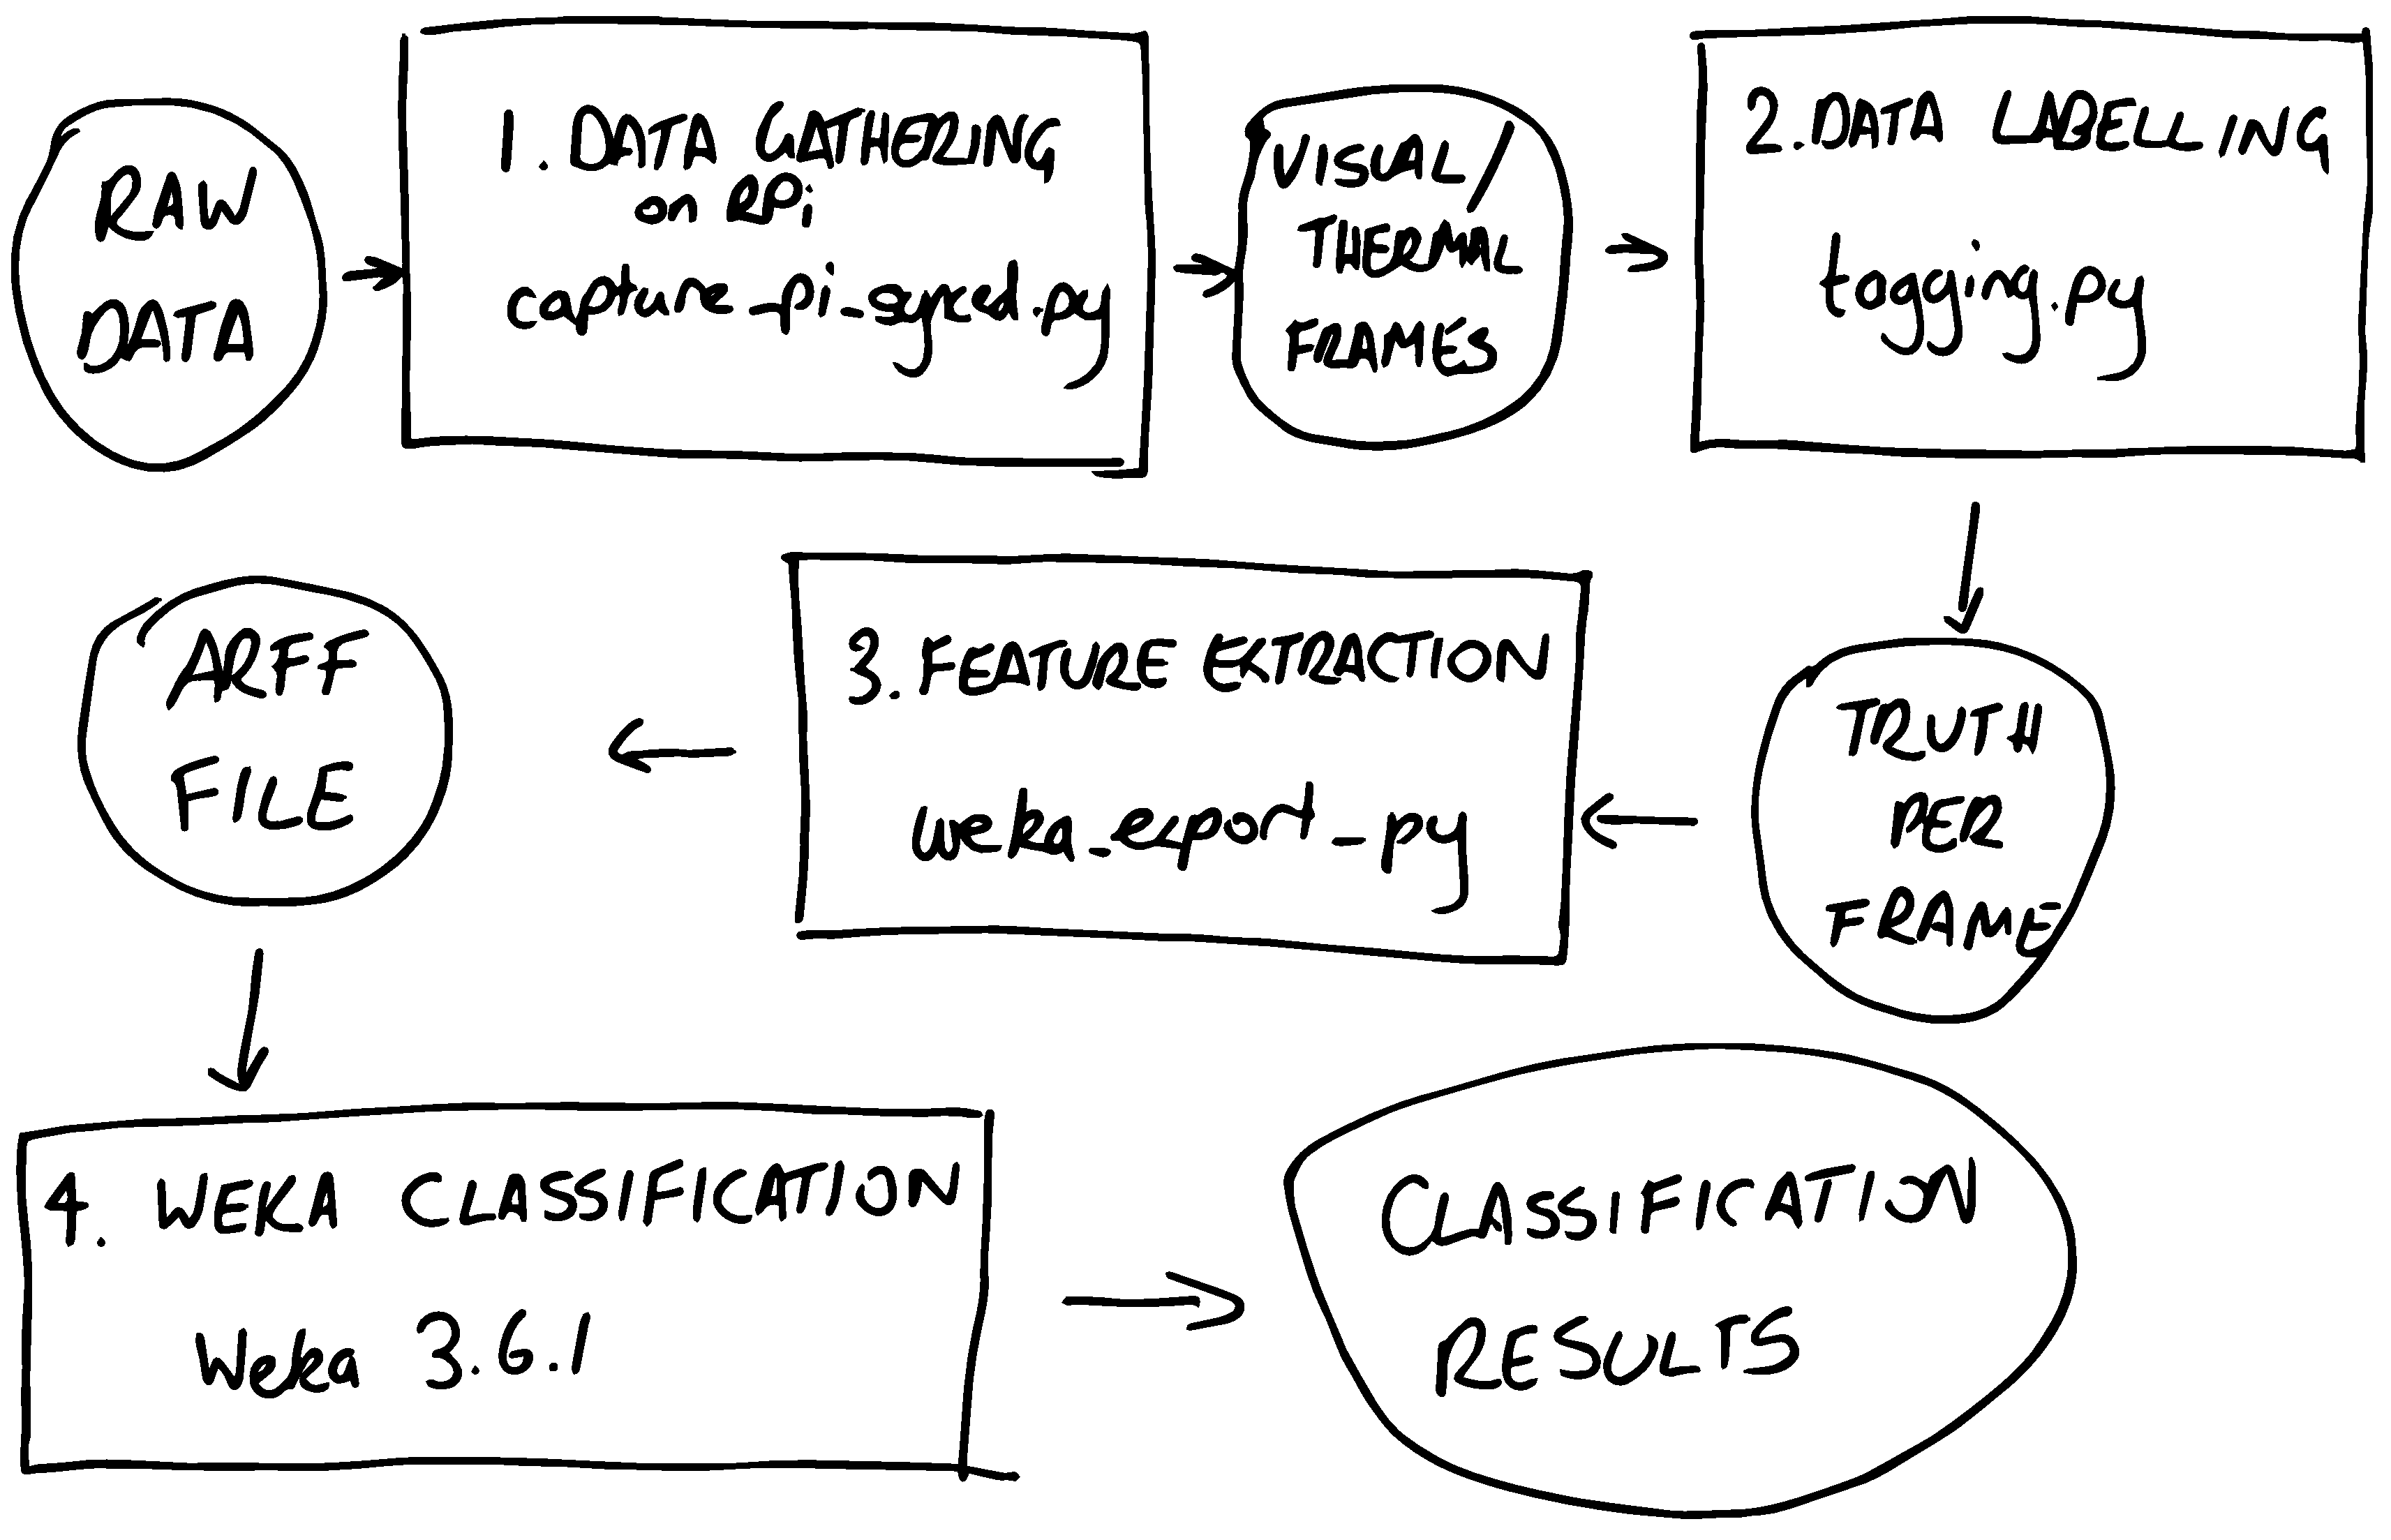
\includegraphics[width=0.95\textwidth]{../diagrams/temp/method-flowchart.pdf}
\caption{Flowchart of processing}
\label{fig:methods:flowchart}
\end{figure}

\subsection{Data gathering}
As the camera and the Arduino are directly plugged into the Raspberry Pi, all data capture is performed on-board through SSH, with the data being then copied of the Pi for later processing. To perform this capture, the main script used is \texttt{capture\_pi\_synced.py}.

\texttt{capture\_pi\_synced.py} takes two parameters on the command line; the name of the capture output, and the number of seconds to capture. By default, it always captures at 2Hz. The script initializes the \texttt{picamera} library, then passes a reference to it to the \texttt{capture\_synced} function within the \texttt{Visualizer} class. The class will then handle the sending of commands to the Arduino to capture data in concert with taking still frames with the Raspberry Pi's camera.

When the script runs, it creates a folder with the name specified, storing inside a file named \texttt{output\_thermal.hcap} containing the thermal capture, and a sequence of files with the format \texttt{video-\%09d.jpg}, corresponding to each visual capture frame.

\subsection{Data labeling}
Once this data capture is complete, the data is copied to a more powerful computer for labeling. The utility \texttt{tagging.py} is used for this stage. This script is passed the path to the capture directory, and the number of frames at the beginning of the capture that are guaranteed to contain no motion. This utility will display frame by frame each visual and thermal capture together, as well as the computed feature vectors (based on a background map created from the first $n$ frames without motion).

The user is then required to press one of the number keys on their keyboard to indicate the number of people present in this frame. This number will be recorded in a file called \texttt{truth} in the capture directory. The next frame will then be displayed, and the process continues. This utility enables the quick input of the ground truth of each capture, making the process more efficient.

\subsection{Feature extraction and data conversion}
Once the ground truth data is available, it is now possible to utilize the data to perform various classification tests. For this, we use version 3.6.11 of the open-source Weka toolkit \cite{Weka}, which provides easy access to a variety of machine learning algorithms and the tools necessary to analyze their effectiveness.

To enable the use of Weka, we export the ground truth and extracted features to Weka Attribute-Relation File Format (ARFF) for processing. \texttt{weka\_export.py} takes two parameters, a comma-separated list of different experiment directories to pull ground truth and feature data from, and the number of frames at the beginning of each capture that can be considered as ``motionless.'' With this information, a CSV-file file is generated on which the heading from \Fref{lst:method:arff} is added for Weka to recognize.

\begin{listing}
\centering
\begin{minted}[fontsize=\footnotesize,frame=single,breaklines=true]{latex}
@RELATION persondata

@ATTRIBUTE npeople  {0,1,2,3} % Or attribute could be numeric using "NUMERIC"
@ATTRIBUTE numactive   NUMERIC
@ATTRIBUTE numconnected  NUMERIC
@ATTRIBUTE sizeconnected   NUMERIC

@DATA
\end{minted}
\caption{ARFF Header}
\label{lst:methods:arff}
\end{listing}

\subsection{Running Weka Tests}
Once the ARFF file is generated, it is then possible to open the file in Weka for processing. Weka provides a variety of algorithms, but we choose a specific subset of algorithms based on those present in the Thermosense paper \cite{beltran2013thermosense}, as well others that we believe adequately represent the different approaches to classification.

We perform the following Weka classification tests on the dataset;

\begin{landscape}
\begin{table}
\centering
\begin{tabular}{|l|l|p{125mm}|}
\hline
\textbf{Type} & \textbf{Attribute} & \textbf{Weka Class} \& \textbf{Parameters} \\ \hline

Neural Net & Nominal, Numeric & \texttt{weka.classifiers.functions.MultilayerPerceptron \newline -L 0.3 -M 0.2 -N 500 -V 0 -S 0 -E 20 -H a} \\ \hline

K-Neareast Neighbours & Nominal, Numeric & \texttt{weka.classifiers.lazy.IBk \newline -K 1 -W 0 \newline -A "weka.core.neighboursearch.LinearNNSearch -A \textbackslash"weka.core.EuclideanDistance -R first-last\textbackslash""} \\ \hline

Naive Bayes & Nominal & \texttt{weka.classifiers.bayes.NaiveBayes} \\ \hline

Support Vector Machine & Nominal & \texttt{weka.classifiers.functions.SMO \newline -C 1.0 -L 0.001 -P 1.0E-12 -N 0 -V -1 -W 1 \newline -K "weka.classifiers.functions.supportVector.PolyKernel -C 250007 -E 1.0"} \\ \hline

Decision Tree & Nominal & \texttt{weka.classifiers.trees.J48 \newline -C 0.25 -M 2} \\ \hline

Entropy Distance & Nominal & \texttt{weka.classifiers.lazy.KStar \newline -B 20 -M a} \\ \hline % TODO: Check that entropy distance

Linear Regression & Numeric & \texttt{weka.classifiers.functions.LinearRegression \newline -S 0 -R 1.0E-8} \\ \hline

Decision Stump & Numeric & \texttt{weka.classifiers.trees.DecisionStump} \\ \hline
\end{tabular}
\caption{Weka classifiers used with parameters}
\label{tab:methods:params}
\end{table}
\end{landscape}

For those tests that are ``nominal,'' the \texttt{npeople} attribute was set to \texttt{\{0,1,...,n\}} where $n$ is the maximum number of people detected in the classification data. For those tests that are ``numeric,'' \texttt{npeople} was set to \texttt{NUMERIC}. For all tests, we use 10-fold cross-validation to validate our results.

As the data we are using is based on real experiments, the number of frames which are classified as each class may be unbalanced, which could cause the classification results to be affected. To that end, for each classification technique, we both classify the data in its raw, unbalanced form, and we also uniformly re-sample the \texttt{npeople} parameter using \texttt{weka.filters.supervised.instance.Resample -B 1.0 -S 1 -Z 100.0} in the pre-processing stage.


\section{Classifier Experiment Set 1 Setup}
The first experiment performed with the prototype described in the previous chapter was set out as indicated in \Fref{fig:exps:3setup}. This experiment involved 3 people, who entered the scene and either remained standing, or sat once they arrived in their positions. The following scripts were observed;

\begin{enumerate}
\item (Remained standing) One person walks in, stands in center, walks out of frame.
\item (Remained standing) One person walks in, joined by another person, both stand there, one leaves, then another leaves.
\item (Remained standing) One person walks in, joined by one, joined by another, all stand there, one leaves, then another, then another.
\item (Remained standing) Two people walk in simultaneously, both stand there, both leave simultaneously.
\item (Sitting) One person walks in, sits in center, moves to right, walks out of frame.
\item (Sitting) One person walks in, joined by another person, both sit there, they stand and switch chairs, one leaves, then another leaves.
\item (Sitting) One person walks in, joined by one, joined by another, they all sit there, one leaves, then another, then another.
\item (Sitting) Two people walk in, both sit there, both leave.
\end{enumerate}

In these experiments people moved slowly and deliberately, making sure there were large pauses between changes of action. The people involved were of average height, wearing various clothing. The room was cooled to 18 degrees for these experiments.

Each experiment was recorded with a thermal-visual synchronization at 1Hz over approximately 60 second intervals. Each experiment had 10-15 frames at the beginning where nothing was within the view of the sensor to allow the thermal background to be calculated. Each frame generated from these experiments was manually tagged with the ground truth value of its occupancy using the script mentioned previously.

The resulting features and ground truth were combined and exported to ARFF allowing the Weka machine learning program to analyze them. This data was analyzed with the feature vectors always being considered numeric data and with the ground truth considered both numeric and nominal (nominal being \texttt{{0,1,2,3}}). All previously mentioned classification algorithms were run against the data set.


\begin{landscape}
 \begin{figure}
 \centering
 % TODO: Proper merging of these figures
 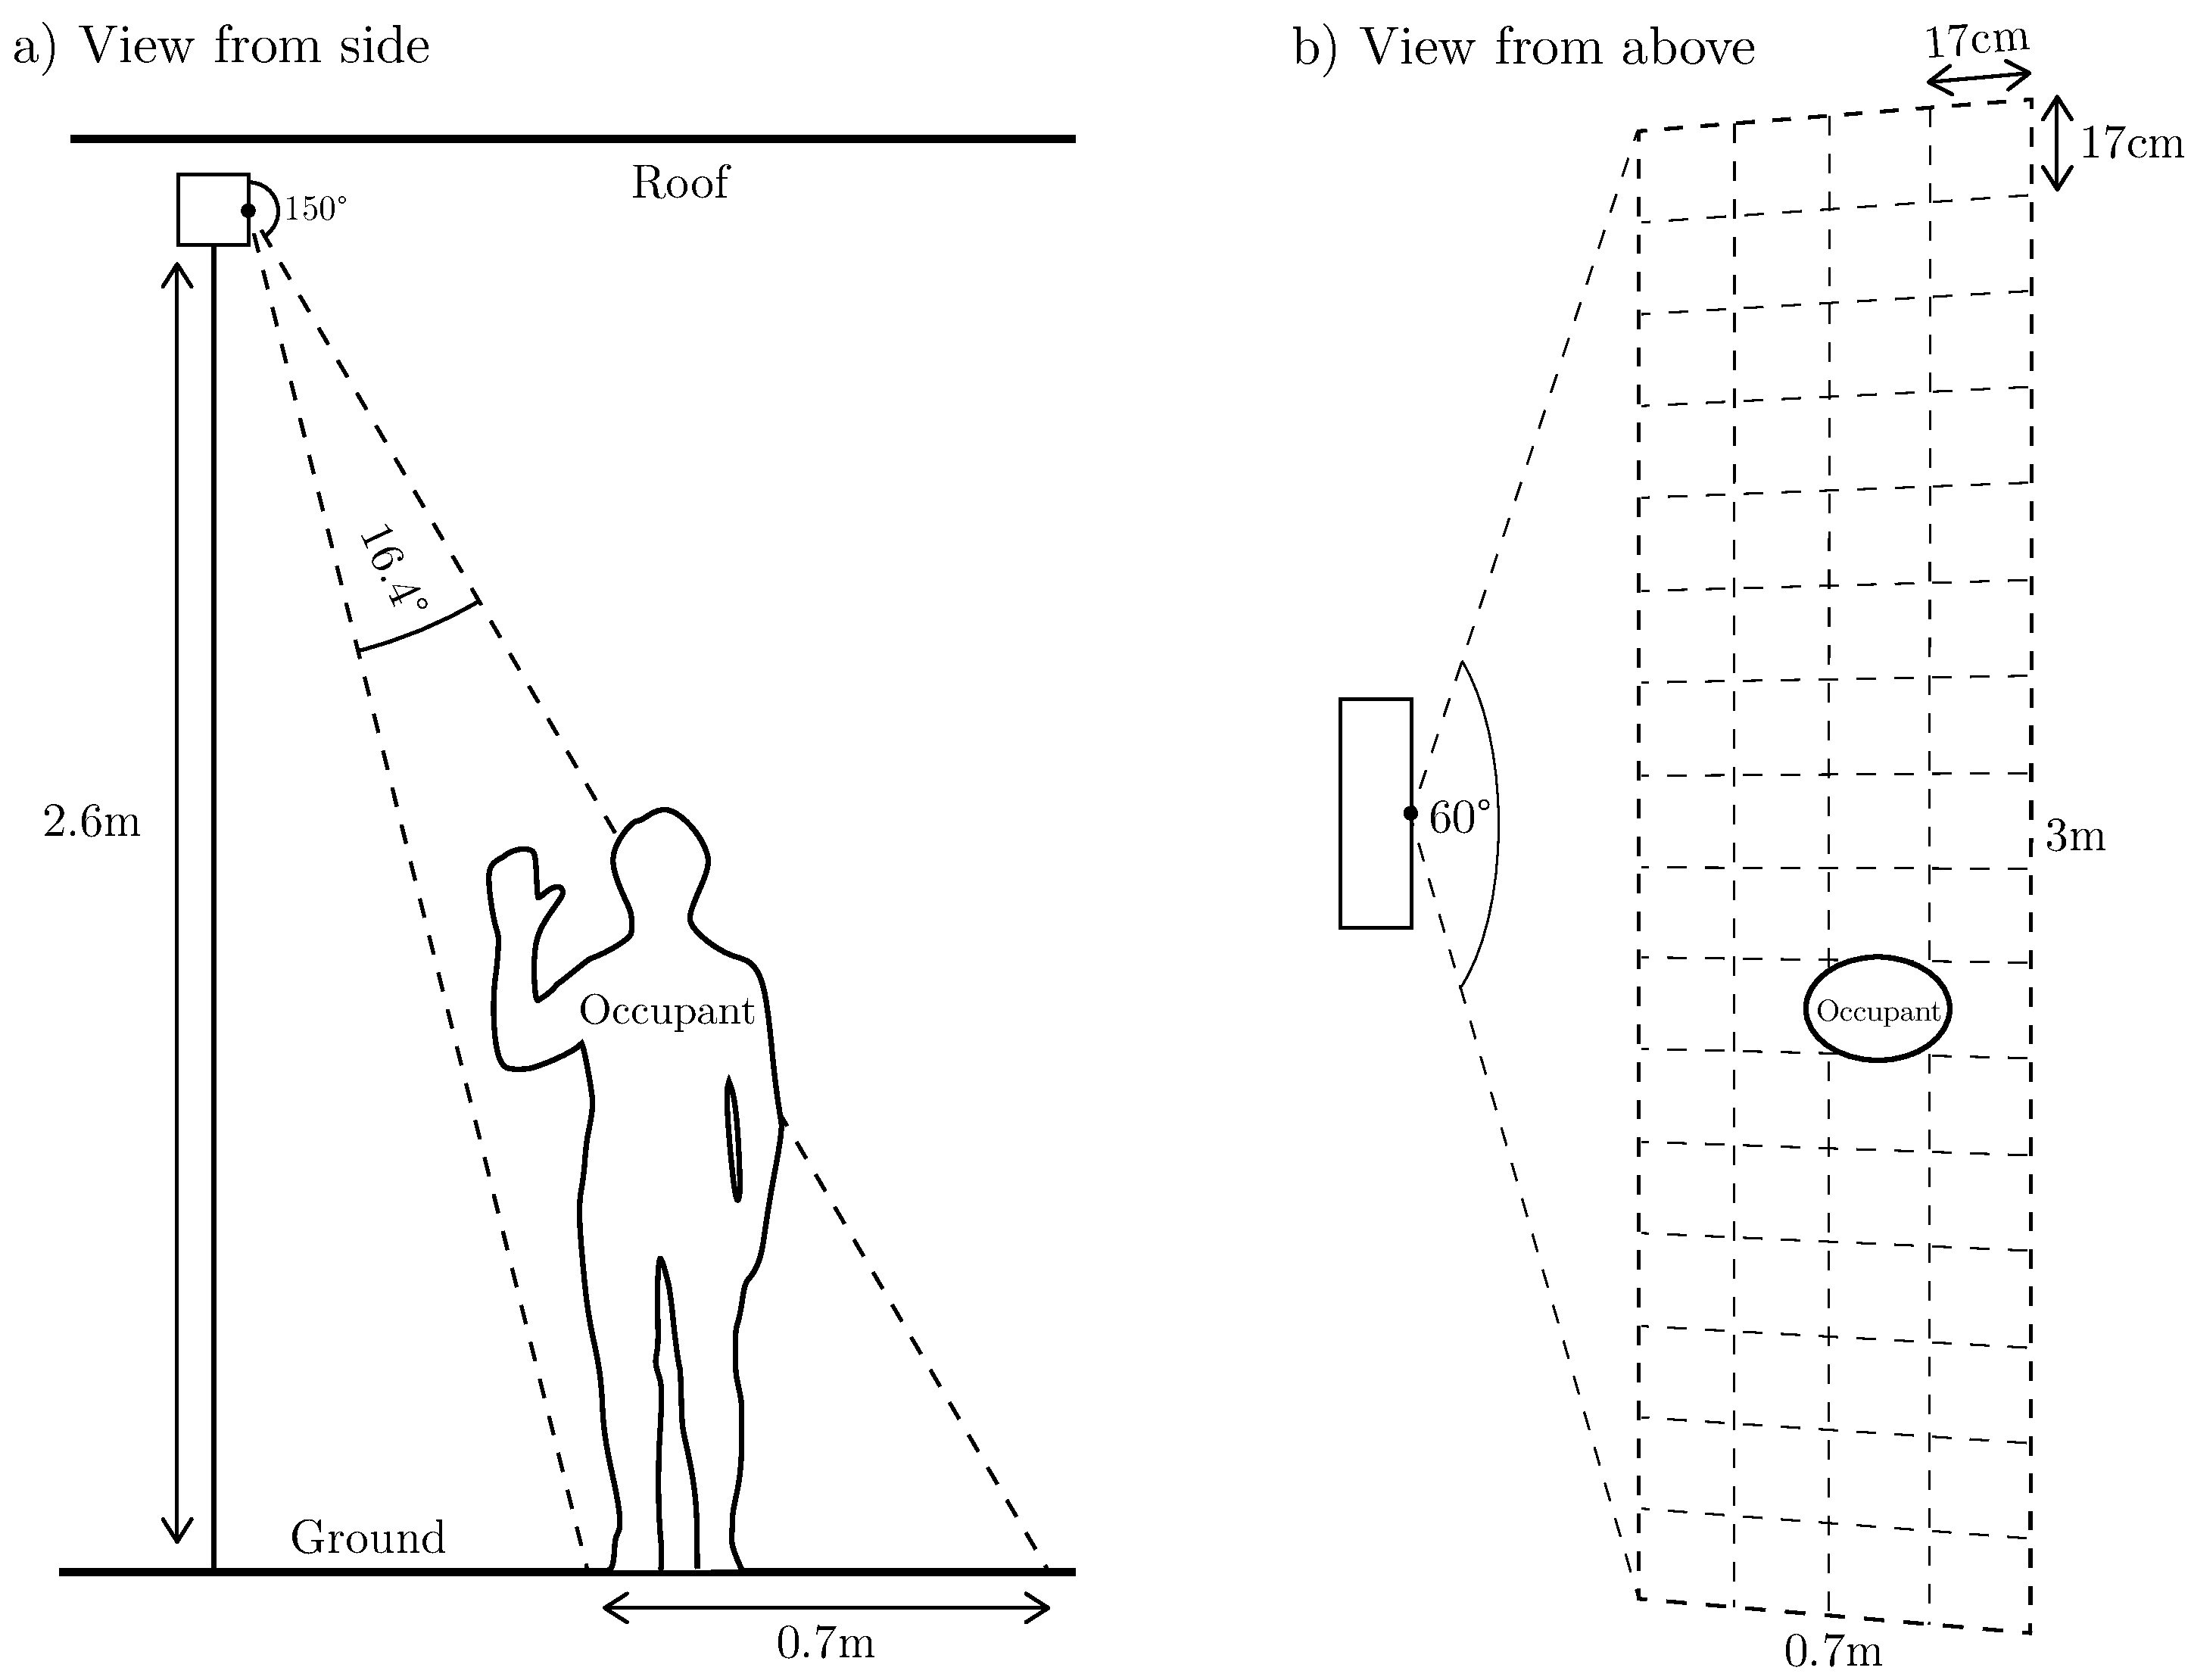
\includegraphics[height=\textheight]{../diagrams/third-exp-setup2.pdf}
 \caption{Classifier Experiment Set 1 Setup}
 \label{fig:exps:3setup}
 \end{figure}
\end{landscape}

 \ifcsdef{mainfile}{}{\bibliography{../references/primary}}
\end{document}
